\subsection{Algorytm mediana median}
Algorytm wygląda następująco:
\begin{verbatim}
findK(S, k);
    if |S| < 50 then
        sort(S);
        return S[k];
    S1, S2, ... Sn/5 = split(S) // podziel S na 5-elementowe podzbiory;
    sort(S1); ... sort(Sn/5);
    Q = {median(S1), ..., median(Sn/5)}
    m = findK(Q, n/10)
    S1 = {x in S: x < M};
    S2 = {x in S: x = M};
    S3 = {x in S: x > M};
    if (|S1| ≥ k)
        return select(S1, k);
    if (|S1| + |S2| ≥ k)
        return M;
    return select(S3, k-|S1|-|S2|);
\end{verbatim}


\subsection{Złożoność}
Kluczową obserwacją jest, że \( \abs{S_1}, \abs{S_3} \leq \frac{3}{4}n \).
Posortowane 5-elementowe podzbiory można przedstawić jak na rysunku poniżej:
\begin{figure}[H]
    \centering
    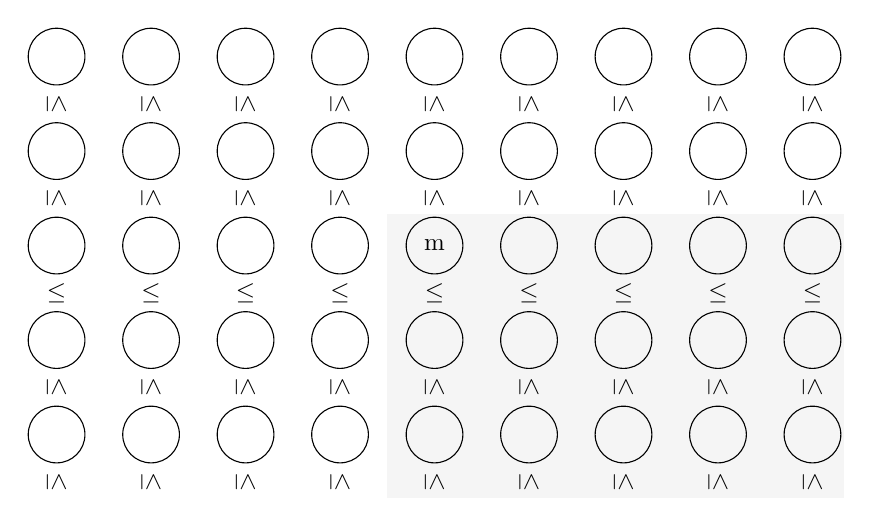
\begin{tikzpicture}[scale=1, every node/.style={scale=0.9}]
  \def\rows{5}
  \def\cols{9}
  \def\cellsize{1.2}

  \filldraw[fill=gray!30, opacity=0.25, draw=none]
    (5*\cellsize - 0.6, -3*\cellsize + 0.4) rectangle
    (9*\cellsize + 0.4, -6*\cellsize + 0.4);

  \foreach \i in {1,...,\rows} {
    \foreach \j in {1,...,\cols} {
      \pgfmathsetmacro\x{\j*\cellsize}
      \pgfmathsetmacro\y{-\i*\cellsize}
      \node[circle, draw, minimum size=8mm] (c\i\j) at (\x,\y) {};
      \ifnum\i=3
        \ifnum\j=5
          \node at (\x,\y) {m};
        \fi
        \node at (\x,\y - 0.6) {\( \leq \)};
      \else
        \node at (\x,\y - 0.6) [rotate=-90]  {\( \leq \)};
      \fi
    }
  }
\end{tikzpicture}
\end{figure}
Elementy prawej dolnej ćwiartki są nie mniejsze niż \( m \), więc \( S_1 \) musi zawierać się w pozostałych trzech ćwiartkach. 
Analogicznie elementy lewej górnej ćwiartki są nie większe niż \( m \), więc \( S_4 \) również musi mieścić się w trzech ćwiartkach. 

Złożoność algorytmu jest opisana równaniem:
\[ T(n) \leq c, dla n < 50 \]
\[ T(n) \leq T(n/5) + T(3/4 n) + c \cdot n,\; n \geq 50 \]
Można pokazać indukcyjnie, że \( T(n) \leq 20 \cdot c \cdot n = \Theta(n) \).

Wynika to również z twierdzenia: \\
Jeśli \( c_i > 0, i = 1, \dots, m, \sum_{i=1, \dots, m} c_i < 1 \), to rozwiązanie
równania
\[ T(n) =\sum_{i=1, \dots, m} T(c_i \cdot n) + \Theta(n) \]
spełnia \( T(n) = \Theta(n) \).

Dlaczego magiczne piątki? \\
Dla trójek równanie rekurencyjne jest postaci
\[ T(n) = T(n/3) + T(2n/3) + O(n), \]
a \( \frac{1}{3} + \frac{2}{3} \not< 1 \) i jego rozwiązaniem jest \( T(n) = \Theta(n \log n) \).
Jeśli chodzi o siódemki, złożoność jest taka sama jak w przypadku piątek, jednak posortowanie zbiorów 7-elementowych wymaga niewątpliwie większej liczby porównań niż zbiorów 5-cio elementowych.
Ot i cała magia